\documentclass
[
  draft    = true,
  fontsize = 11pt,
  parskip  = half-,
  BCOR     = 0pt,
  DIV      = 11,
  ngerman,
  dvipsnames
]
{scrartcl}

% Standardpakete
\usepackage{fixltx2e}
\usepackage[utf8]{inputenc}
\usepackage[T1]{fontenc}
\usepackage{lmodern}
\usepackage{babel}
% Zusatzpakete
\usepackage{amsmath}
\usepackage{amssymb}
\usepackage{tikz}


% --------
% function
% --------
%
% #1  xshift
% #2  function (term)
% #3  ymin
% #4  ymax
%
\newenvironment{function}[4]
{%
  \begin{scope}[xshift=#1]
    % Funktionsgleichung
    \node[above right] at (-6, #4) {#2};
    % Koordinatenachsen
    \draw[line width=0.8pt, ->, >=latex] (-6, 0) -- (6, 0);
    \draw[line width=0.8pt, ->, >=latex] (0, #3) -- (0, #4);
    % Funktionen
    \begin{scope}
      \clip (-6, #3) rectangle (6, #4);
}%
{%
    \end{scope}   
  \end{scope}
}

% -----
% fplot
% -----
%
% #1  file with coordinates
%
\newcommand{\fplot}[1]
{%
  \draw[line width=0.6pt, draw=blue] plot[smooth] file{#1};
}


% ------------------------------------------------------------------------------
\begin{document}
% ------------------------------------------------------------------------------

% ----------------------------------------
\section*{Graphen ausgewählter Funktionen}
%-----------------------------------------
\begin{center}
  \newcommand{\ymin}{-5}
  \newcommand{\ymax}{5}
  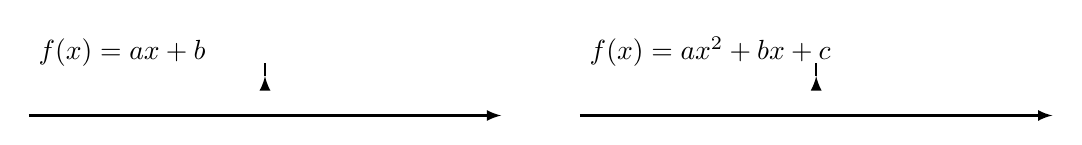
\begin{tikzpicture}[scale=0.5]
    \begin{function}{-7cm}{$f(x)=ax+b$}{\ymin}{\ymax}
      \fplot{octave/poly1.xy}
    \end{function}
    \begin{function}{7cm}{$f(x)=ax^{2}+bx+c$}{\ymin}{\ymax}
      \fplot{octave/poly2.xy}
    \end{function}
  \end{tikzpicture}
\end{center}

\begin{center}
  \newcommand{\ymin}{-5}
  \newcommand{\ymax}{5}
  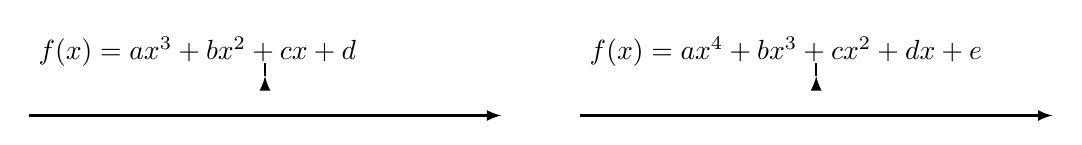
\begin{tikzpicture}[scale=0.5]
    \begin{function}{-7cm}{$f(x)=ax^{3}+bx^{2}+cx+d$}{\ymin}{\ymax}
      \fplot{octave/poly3.xy}
    \end{function}
    \begin{function}{7cm}{$f(x)=ax^{4}+bx^{3}+cx^{2}+dx+e$}{\ymin}{\ymax}
      \fplot{octave/poly4.xy}
    \end{function}
  \end{tikzpicture}
\end{center}

\begin{center}
  \newcommand{\ymin}{-3}
  \newcommand{\ymax}{4}
  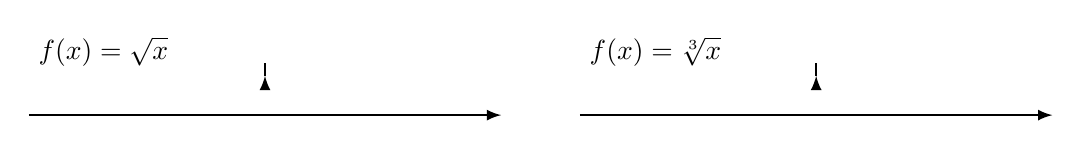
\begin{tikzpicture}[scale=0.5]
    \begin{function}{-7cm}{$f(x)=\sqrt{x}$}{\ymin}{\ymax}
      \fplot{octave/sqr2.xy}
    \end{function}
    \begin{function}{7cm}{$f(x)=\sqrt[3]{x}$}{\ymin}{\ymax}
      \fplot{octave/sqr3.xy}
    \end{function}
  \end{tikzpicture}
\end{center}

\begin{center}
  \newcommand{\ymin}{-2}
  \newcommand{\ymax}{4}
  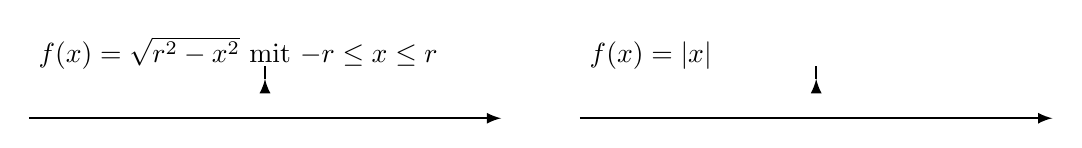
\begin{tikzpicture}[scale=0.5]
    \begin{function}{-7cm}{$f(x)=\sqrt{r^{2}-x^{2}}$ mit $-r\leq x\leq r$}{\ymin}{\ymax}
      \fplot{octave/circ.xy}
    \end{function}
    \begin{function}{7cm}{$f(x)=|x|$}{\ymin}{\ymax}
      \fplot{octave/absval.xy}
    \end{function}
  \end{tikzpicture}
\end{center}

\begin{center}
  \newcommand{\ymin}{-6}
  \newcommand{\ymax}{6}
  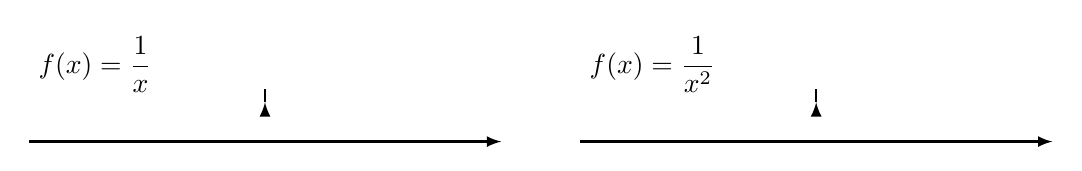
\begin{tikzpicture}[scale=0.5]
    \begin{function}{-7cm}{$\displaystyle f(x)=\frac{1}{x}$}{\ymin}{\ymax}
      \fplot{octave/hyp1-part01.xy}
      \fplot{octave/hyp1-part02.xy}
    \end{function}
    \begin{function}{7cm}{$\displaystyle f(x)=\frac{1}{x^{2}}$}{\ymin}{\ymax}
      \fplot{octave/hyp2-part01.xy}
      \fplot{octave/hyp2-part02.xy}
    \end{function}
  \end{tikzpicture}
\end{center}

\begin{center}
  \newcommand{\ymin}{-6}
  \newcommand{\ymax}{6}
  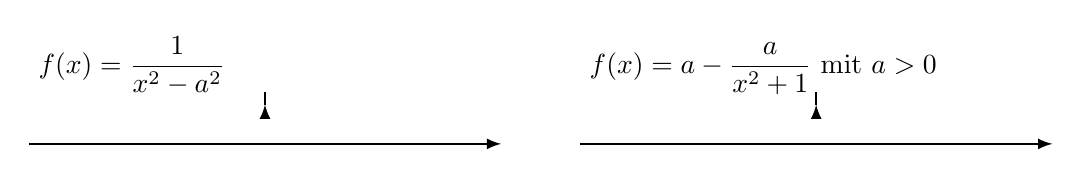
\begin{tikzpicture}[scale=0.5]
    \begin{function}{-7cm}{$\displaystyle f(x)=\frac{1}{x^{2}-a^{2}}$}{\ymin}{\ymax}
      \fplot{octave/pol2-part01.xy}
      \fplot{octave/pol2-part02.xy}
      \fplot{octave/pol2-part03.xy}
    \end{function}
    \begin{function}{7cm}{$\displaystyle f(x)=a-\frac{a}{x^{2}+1}$ mit $a>0$}{\ymin}{\ymax}
      \fplot{octave/valley.xy}
    \end{function}
  \end{tikzpicture}
\end{center}

\begin{center}
  \newcommand{\ymin}{-2}
  \newcommand{\ymax}{6}
  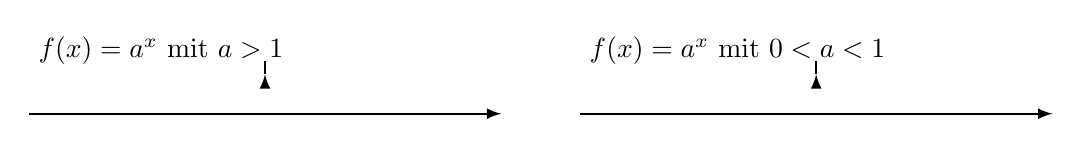
\begin{tikzpicture}[scale=0.5]
    \begin{function}{-7cm}{$f(x)=a^{x}$ mit $a>1$}{\ymin}{\ymax}
      \fplot{octave/exppos.xy}
    \end{function}
    \begin{function}{7cm}{$f(x)=a^{x}$ mit $0<a<1$}{\ymin}{\ymax}
      \fplot{octave/expneg.xy}
    \end{function}
  \end{tikzpicture}
\end{center}

\begin{center}
  \newcommand{\ymin}{-5.5}
  \newcommand{\ymax}{5.5}
  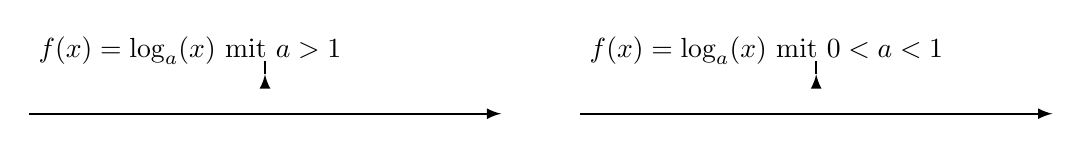
\begin{tikzpicture}[scale=0.5]
    \begin{function}{-7cm}{$f(x)=\log_{a}(x)$ mit $a>1$}{\ymin}{\ymax}
      \fplot{octave/logbig.xy}
    \end{function}
    \begin{function}{7cm}{$f(x)=\log_{a}(x)$ mit $0<a<1$}{\ymin}{\ymax}
      \fplot{octave/logsmall.xy}
    \end{function}
  \end{tikzpicture}
\end{center}

\begin{center}
  \newcommand{\ymin}{-2}
  \newcommand{\ymax}{4}
  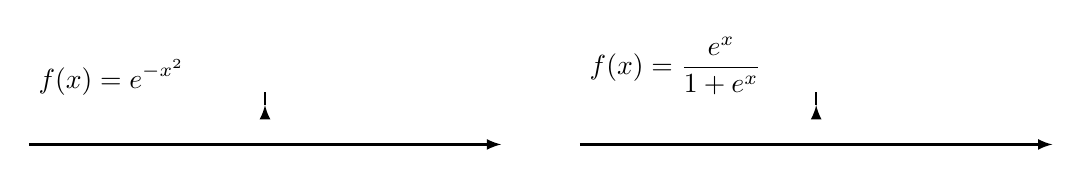
\begin{tikzpicture}[scale=0.5]
    \begin{function}{-7cm}{$\displaystyle f(x)=e^{-x^{2}}$}{\ymin}{\ymax}
      \fplot{octave/expquad.xy}
    \end{function}
    \begin{function}{7cm}{$\displaystyle f(x)=\frac{e^{x}}{1+e^{x}}$}{\ymin}{\ymax}
      \fplot{octave/sig.xy}
    \end{function}
  \end{tikzpicture}
\end{center}

\begin{center}
  \newcommand{\ymin}{-2}
  \newcommand{\ymax}{2}
  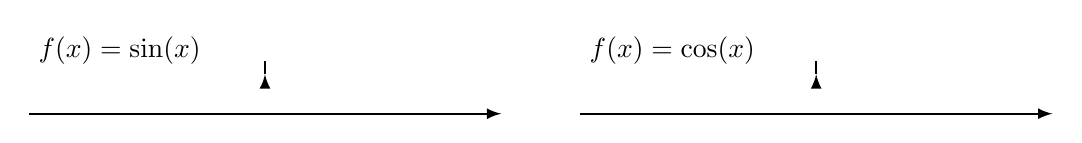
\begin{tikzpicture}[scale=0.5]
    \begin{function}{-7cm}{$f(x)=\sin(x)$}{\ymin}{\ymax}
      \fplot{octave/sinus.xy}
    \end{function}
    \begin{function}{7cm}{$f(x)=\cos(x)$}{\ymin}{\ymax}
      \fplot{octave/cosinus.xy}
    \end{function}
  \end{tikzpicture}
\end{center}

\begin{center}
  \newcommand{\ymin}{-5.5}
  \newcommand{\ymax}{5.5}
  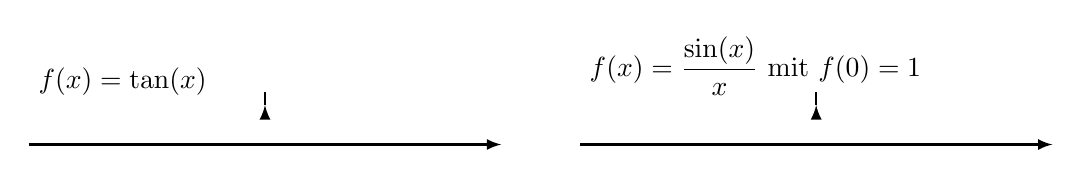
\begin{tikzpicture}[scale=0.5]
    \begin{function}{-7cm}{$f(x)=\tan(x)$}{\ymin}{\ymax}
      \fplot{octave/tangens-part01.xy}
      \fplot{octave/tangens-part02.xy}
      \fplot{octave/tangens-part03.xy}
      \fplot{octave/tangens-part04.xy}
      \fplot{octave/tangens-part05.xy}
      \fplot{octave/tangens-part06.xy}
      \fplot{octave/tangens-part07.xy}
    \end{function}
    \begin{function}{7cm}{$\displaystyle f(x)=\frac{\sin(x)}{x}$ mit $f(0)=1$}{\ymin}{\ymax}
      \fplot{octave/cardsin.xy}
    \end{function}
  \end{tikzpicture}
\end{center}

% ------------------------------------------------------------------------------
\end{document}
% ------------------------------------------------------------------------------

